\documentclass[aps, prl, letterpaper, twocolumn, superscriptaddress, notitlepage, 10pt]{revtex4-1}
\usepackage{times}

% use these settings for a more reader-friendly version
%\documentclass[aps, pra, a4paper, 11pt, onecolumn, nofootinbib, superscriptaddress, tightenlines, notitlepage, longbibliography]{revtex4-1}

%------------------------------------------------------------------------------------------------------------%
% Packages
%------------------------------------------------------------------------------------------------------------%

\usepackage{color}
\usepackage{amsmath,amsfonts,amssymb}
\usepackage{graphicx}
\usepackage[caption=false]{subfig}
\usepackage{enumerate}
\usepackage{mathrsfs}


%\usepackage{epstopdf} % to include .eps graphics files with pdfLaTeX

\usepackage[pdfpagelabels,pdftex,bookmarks,breaklinks]{hyperref}
\definecolor{darkblue}{RGB}{0,0,127} % choose colors
\definecolor{darkgreen}{RGB}{0,150,0}
\hypersetup{colorlinks, linkcolor=darkblue, citecolor=darkgreen, filecolor=red, urlcolor=blue}
\hypersetup{pdfauthor={Simon Burton, Courtney G. Brell, Steven T. Flammia}}
\hypersetup{pdftitle={Classical Simulation of Quantum Error Correction in a Fibonacci Anyon Code}}

\usepackage[normalem]{ulem}

%------------------------------------------------------------------------------------------------------------%
% Macros
%------------------------------------------------------------------------------------------------------------%

\newcommand{\Eref}[1]{Eq.~(\ref{#1})}
\newcommand{\Fref}[1]{Fig.~\ref{#1}}
\newcommand{\Aref}[1]{Appendix~\ref{#1}}

\newcommand{\e}{\mathrm{e}}
\newcommand{\vac}{\mathbb{I}}

\newcommand{\ket}[1]{|{#1}\rangle}
\newcommand{\expect}[1]{\langle{#1}\rangle}
\newcommand{\bra}[1]{\langle{#1}|}
\newcommand{\ketbra}[2]{\ket{#1}\!\bra{#2}}
\newcommand{\braket}[2]{\langle{#1}|{#2}\rangle}
\newcommand{\proj}[1]{\ketbra{#1}{#1}}

\newcommand{\cggb}[1]{\textcolor{blue}{#1}}
\newcommand{\simon}[1]{\textcolor{red}{#1}}

\newcommand{\F}{\mathscr{H}} % H or F ?
\newcommand{\C}{\mathbb{C}}
\newcommand{\R}{\mathbb{R}}
\newcommand{\A}{\mathcal{A}}

%------------------------------------------------------------------------------------------------------------%
\begin{document}

\title{Classical Simulation of a Modular Functor}

\author{Simon Burton}
\affiliation{Centre for Engineered Quantum Systems, School of Physics, 
The University of Sydney, Sydney, Australia}
\author{Courtney G.\ Brell}
\affiliation{Institut f\"{u}r Theoretische Physik, Leibniz Universit\"{a}t Hannover, 
Appelstra\ss{}e 2, 30167 Hannover, Germany}
\author{Steven T.\ Flammia}
\affiliation{Centre for Engineered Quantum Systems, School of Physics, 
The University of Sydney, Sydney, Australia}

\date{\today}

\maketitle

%------------------------------------------------------------------------------------------------------------%

\onecolumngrid
\appendix



The goal here is to describe the algorithm for
computing charge contained regions built from 
arbitrary collection of tiles.
To do this we first describe our approach
to topological quantum field theory,
then we discuss the data structure 
(combinatorial curve diagrams) and the algorithm
that operates on these structures.

%We give an informal introduction to
%anyonic topological quantum
%field theory in $(2+1)$-dimensions.
%See \cite{beverland2014} for a similar treatment.
%Note that these theories give rise to
%\emph{doubled} anyonic charges, and so
%the Fibonacci example in the main text simulates
%one half of such a system. % MEH!

%
% ~~~~~~~~~~~~~~~~~~~~~~~~~~~~~~~~~~~~~~~~~~~~~~~~~~~~~~~~~~~~~~~~~~~~~~~~~~~~
%

%\section{Topological quantum field theory}
\section{A TQFT warmup}

In two spacial dimensions, particle exchange is
captured by the braid group.
World lines of such particles 
become tangled (braided) in $(2+1)$-dimensions.
For example, three particle statistics is captured
by the braid group on three strands $B_3.$
This group is generated by elements $\sigma_1$
and $\sigma_2$ which we represent pictorially as:
\begin{center}
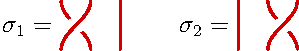
\includegraphics[]{pic-braid-group.pdf}
\end{center}

These pictures make clear how the group
multiplication works, for example:
\begin{center}
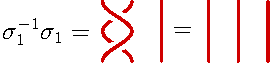
\includegraphics[]{pic-braid-group-1.pdf}
\end{center}
\begin{center}
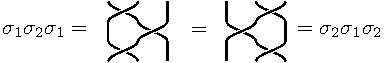
\includegraphics[]{pic-braid-relation.pdf}
\end{center}


These diagrams are to be understood up to
continuous deformation of the ambient space.
That is, we allow the ambient $(2+1)$-dimensional
space with these worldlines subtracted to be continuously
deformed.
At the top and bottom of this space is 
a $2$-dimensional space (a disc) with holes in it.
Such a closed disc with $n$ holes we denote as $D_n.$
So this is how we arrive at modelling the system as
a disc with holes in it.
The observables of the system measure charge within
a region bounded by a directed closed curve.
\begin{center}
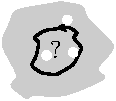
\includegraphics[]{pic-observable.pdf}
\end{center}

The defining feature of an Abelian anyon theory
is that the state is completely determined once
we measure the charge of each hole.
In the language of the toric code (homology),
logical operators (1-chains)
cancel where they overlap
with opposite orientation:
\begin{center}
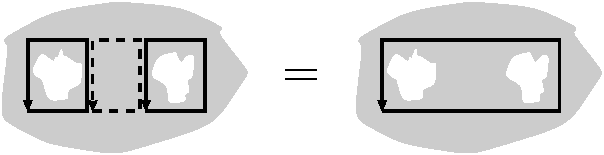
\includegraphics[width=0.4\columnwidth]{pic-abelian.pdf}
\end{center}

This is not at all the case in general;
for non-Abelian theories there can be extra
degrees of freedom associated with these
observables. For example, in
a system supporting Fibonacci anyons,
we can have two Fibonacci anyons with total
charge either vacuum or Fibonacci:
\begin{center}
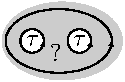
\includegraphics[]{pic-fusion.pdf}
\end{center}
so the state space of two fibonacci anyons
is $2$-dimensional.
Such a space associated with observing total charge
of multiple anyons is called the \emph{fusion} space
of those charges.

These observables satisfy various relations,
but in particular, non-overlapping observables commute.
So if we nest a maximal set of these observables together
we can pin-down a basis for the fusion space.
Such a nesting is tree-like, and if we confuse the distinction
between holes and observables, this gives rise to the
fusion tree notation.
\begin{center}
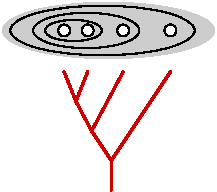
\includegraphics[]{pic-tree-0.pdf}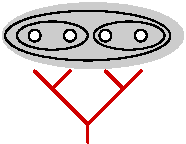
\includegraphics[]{pic-tree-1.pdf}
\end{center}

Given a disc with $n$ holes, we define the \emph{mapping
class group} $MCG(D_n)$ as the group of topological
symmetries (homeomorphisms) of the space $D_n,$
modulo continuous deformations (isotopy).
Such symmetries we require to fix the boundary
of the disc, but not necessarily to fix the holes.
Elements $f\in MCG(D_n)$ will also act on anything that
resides in $D_n.$ 
In particular, if we draw a line
connecting the holes:
\begin{center}
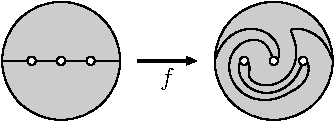
\includegraphics[]{pic-twist.pdf}
\end{center}

Such an embedding $c : [0, 1] \to D$ with $c(0), c(1) \in \partial D$
and touching all holes in $D_n$ we call a \emph{curve diagram}~\cite{Dehornoy2002},
(or just a \emph{curve} when the context is clear).

We can think of braids acting on states in a Schrodinger picture,
or alternatively, elements of the mapping class group acting on
observables in a Heisenberg picture:
\begin{center}
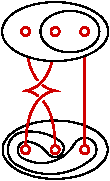
\includegraphics[]{pic-interaction.pdf}
\end{center}

We would hope that the groups $B_n$ and $MCG(D_n)$ are
isomorphic, and this is indeed the case~\cite{Kassel2010}.
One can see this as follows. Dragging the space $D_n$ along
a braid creates a deformation, the end point of which is a
homeomorphism in $MCG(D_n).$ Going the other direction,
given $f\in MCG(D_n)$ and a curve diagram $c,$ we think of
pulling the ends of $f\circ c$, thereby moving (braiding) the holes,
until we are back at the original curve $c.$

%This discussion makes it clear we have picked out a
%specific curve $c$ that we use as a reference point for
%other curves. 

The importance of this isomorphism: the simulation
algorithm calculates outcomes of observations. This
boils down to a change of basis, to one that includes
the required observable.
$F$-moves allow us to re-associate observables along
a curve diagram. The mapping class group acts
transitively on curve diagrams (\emph{why??}).

%
% ~~~~~~~~~~~~~~~~~~~~~~~~~~~~~~~~~~~~~~~~~~~~~~~~~~~~~~~~~~~~~~~~~~~~~~~~~~~~
%

\section{Modular Functors}

The definition of a Modular functor appears to
be well motivated physically....
Unfortunately, there are many such definitions
in the literature, and little work has been done
on the connection between these different axiomatizations
(\cite{Bartlett2015} section 1.2 and 1.3).
In particular, what physicists call Anyon theory,
and mathematicians call a Modular Tensor Category,
has not been established to correspond exactly
(bijectively) to any of these modular functor
variants.

As in algebraic topology, we wish to extract
algebraic information about topological objects.
This can be viewed as a kind of representation theory
of topological objects: homeomorphisms of surfaces.

We list the axioms for a 
\emph{2-dimensional unitary topological modular functor}.
 % abbreviated as \emph{MF}.
There are quite alot of details that we leave out,
%For the details of this construction, see
see
\cite{Turaev1994}, \cite{Walker1991} or \cite{Bakalov2000}.
For a more pedestrian treatment, see \cite{Freedman2002simulation} or \cite{Beverland2014}.

For our purposes a \emph{surface} will be a compact
oriented $2$-dimensional manifold with boundary. % smooth or topological ?
We will not require surfaces to be connected.
%Each boundary component is oriented (either explicitly or
%otherwise by using the orientation of the manifold)
By a \emph{hole} of $M$ we mean a component of its boundary. % $\partial M$.
Each hole will inherit the manifold orientation,
contain a distinguished \emph{base point},
and be labelled with
%an element from a finite set $\mathbb{A}=\{1, a, b, c ...\}.$
an element from a (fixed) finite set $\A.$
This is the set of ``anyon labels'', and comes
equiped with a vacuum element $\vac$ 
and an involution $\ \widehat{}\ $ such that $\widehat{\vac}=\vac.$

We will mostly be concerned with \emph{planar} such
surfaces, ie. disc(s) with zero or more holes.
Such surfaces will be given a counterclockwise 
orientation, which induces a clockwise orientation on
any \emph{interior} hole and a counterclockwise orientation
on the \emph{exterior} hole.
\begin{center}
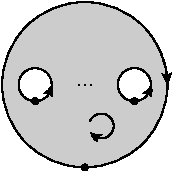
\includegraphics[]{pic-disc.pdf}
\end{center}

A map of surfaces $f:M\to N$ will be understood to be
a topological homeomorphism that preserves
manifold orientation, hole labels, and base points.

A \emph{modular functor} $\F$ associates to every
surface $M$ a finite dimensional complex
vector space $\F(M)$, called the \emph{fusion space} of $M$.
For each map $f:M\to N$
The modular functor associates a
unitary transformation $\F(f) : \F(M)\to\F(N)$
that only depends on the isotopy class of $f.$
Functoriality requires that $\F$
respect composition of maps.

We have the following axioms for $\F.$

{\bf Axiom I.}
The fusion space of an empty surface is one dimensional, 
$\F(\phi) \cong \C.$ % preserves the identity of tensor
For $M_a$ a disc with boundary label $a$ we have
$\F(M_\vac)\cong \C$ and 
$\F(M_a)\cong 0$ for $a\ne \vac.$
For annulus $M_{a,b}$ with boundary labels
$a, b$ we have
$\F(M_{a,\widehat{a}})\cong \C$ and 
$\F(M_{a,b})\cong 0$ for $a\ne \widehat{b}.$

{\bf Axiom II.}
The disjoint union of two surfaces $M$ and $N$ 
is associated with
the tensor product of fusion spaces:
$$
    \F(M\amalg N) \cong \F(M)\otimes \F(N).
$$
This is natural from the point of view of quantum
physics, where the Hilbert space of two disjoint
systems is the tensor product of the space for
each system.

{\bf Axiom III.}
%Gluing.
Denote a surface $M$ with (at least) two holes
labelled $a, b$ as $M_{a,b}$. 
If we constrain $b=\widehat{a}$ 
then we may \emph{glue} these two holes together
to form a new surface $N.$
%Let $N$ be the surface obtained from $M$ by gluing
%these two holes together.
%By this we mean there is a homeomorphism from one
To construct $N$ we choose a homeomorphism from one
hole to the other that maps base point to base point 
and reverses orientation.
Identifying the two holes along this homeomorphism
gives the glued manifold $N.$
%Gluing must reverse the orientation of the two holes
%as well as identifying their base points.
The fusion space of $M_{a,\widehat{a}}$ then embedds unitarily in the fusion
space of $N.$
Moreover, there is an isomorphism called
a \emph{gluing map}:
$$
    \bigoplus_{a\in\A} \F(M_{a,\widehat{a}}) \xrightarrow{\cong} \F(N).
$$
The seam along which gluing occurs can be associated
with an observable as follows.
We take a gluing map $g$. Projectors $P_a$ onto the
summands in the above direct sum:
$$
    P_a: \bigoplus_{b\in\A} \F(M_{b,\widehat{b}}) \to \F(M_{a,\widehat{a}}).
$$
then the observable will be the set of operators $\{P_a g^{-1}\}_{a\in\A}.$

A common operation is to glue two separate surfaces.
We can do this by first taking disjoint union (tensoring
the fusion spaces)
and then gluing.
Here we show this process applied to two surfaces $M$ and $N$. 
\begin{center}
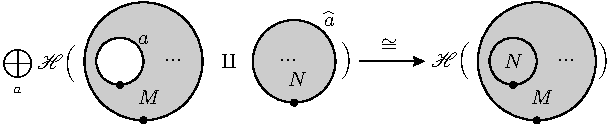
\includegraphics[]{pic-glue.pdf}
\end{center}
We display the surface $N$ with the $\widehat{a}$
boundary on the outside, 
to show more clearly how $N$ fits into $M$.
In the glued manifold we
indicate the placement of $M$ and $N$ and the seam
along which gluing occured,
as well as the identification of base points.

%\emph{XXX show orientation of boundaries ?}
%\emph{XXX displaymath direct sum}
%\emph{XXX $N...$ show ellipses?}

It follows that:
1) a vacuum boundary component may be ``filled-in''
replaced with a disk by gluing.
2) the dimensionality of the fusion space of a torus is the
cardinality of $\A.$ This follows by gluing one end
of an anulus (cylindar) to the other.

%A most important linear map, called an $F-$move,
%As a slightly more complicated example of glueing
%we consider the following two arr
The $F-$move
is constructed from two applications of a
gluing map as follows:

\begin{center}
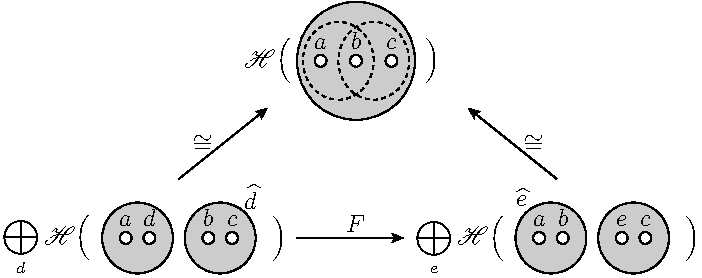
\includegraphics[]{pic-glue-fmove.pdf}
\end{center}

Here we have shown a manifold $M_{abc}$ with 
three labelled boundaries, as well as two separate
ways of gluing pairs-of-pants to get $M.$
%\emph{XXX do we label with $d$ or $\widehat{d}$ ?}

The fusion space of the disc and annulus are
specified by the axioms, and we define the fusion
space of the disc with two holes, or ``pair-of-pants''
as:
\begin{center}
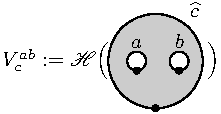
\includegraphics[]{pic-pop.pdf}
\end{center}
Using this notation, the above $F-$move
is a linear map
$$
    F^{abc}_d : \bigoplus_{x\in\A} V^{ab}_x\otimes V^{xc}_d 
        \to \bigoplus_{y\in\A} V^{ay}_d\otimes V^{bc}_y.
$$

%The reverse process of cutting a surface up
%into pair-of-pants induces a direct sum decomposition
%of the fusion space.
Given a manifold $M$ which is
a disc with at least two holes, 
we show how to present $M$ as the glueing of various
pair-of-pants 
(See \cite{Ivanov2001} for more details on this construction,
and \cite{Ghrist2014} for more about Morse theory).
This will yield a decomposition of $\F(M)$ into a direct
sum of fusion spaces of pair-of-pants. % $V_{ab}^c$'s.
%The pair-of-pants can be found using Morse theory.
We proceed using Morse theory.
Note that we need $M$ to be a differentiable manifold for
this to work.
Choose a Morse function (a generic ``height'' function) $h:M\to\R$
such that $h$ is constant on $\partial M,$
and the values of $h$ at different critical points are different.
Now choose a sequence of non-critical values $a_1<a_2<...<a_n$ in $\R$
such that every interval $[a_{i-1}, a_i]$ 
contains exactly one critical value of $h$ and the image
of $h$ lies within $[a_1, a_n].$
%cuts the manifold into pieces $f^{-1}[a,b]$.
Each component of $h^{-1}([a_{i-1}, a_i])$ is then either
an annulus, a disc, or a pair-of-pants depending on the index of (any)
critical point it contains.
We then ``re-glue'' any annuli or discs until there are no more of these
and we have only pair-of-pants.
\begin{center}
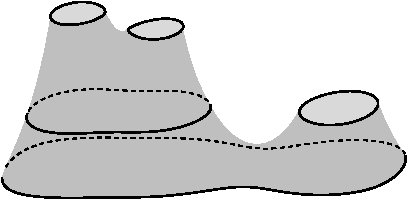
\includegraphics[]{pic-pants.pdf}\ \ \ \ \ \ \ \ 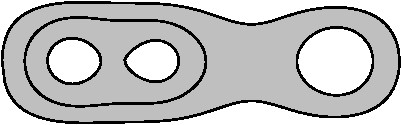
\includegraphics[]{pic-pants-1.pdf}
\end{center}

Clearly such a pair-of-pants decomposition is not unique,
and the goal here is to switch between decompositions,
and in particular, given an observable $\gamma$,
and a given pair-of-pants decomposition, find a sequence
of ``moves'' such that $\gamma$ is in the resulting pair-of-pants
decomposition:
\begin{center}
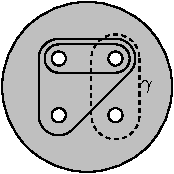
\includegraphics[]{pic-refactor.pdf}
\end{center}

One way to achieve this is via Cerf theory, which is the theory
of how one may deform Morse functions into other Morse functions
and the kind of transitions involved in their critical point structure.
This was the approach used in \cite{Freedman2002simulation}.
In this work we use a simpler method,
which is essentially the same as \emph{skein theory.}
Read on to find out how this works!

%Pair-of-pants decomposition corresponds to a direct sum decomposition of
%the fusion space.
The projectors associated to each cuff commute.
Non-overlapping observables commute.

As we have seen, an oriented simple closed path 
contained in the interior of $M$ can serve as
the seam along which gluing occurs and we call
these paths \emph{observables}.
%Any oriented simple closed path contained in the interior of $M$ we will
%call an \emph{observable}.
%Such a path has no orientation because it 
%lies withing the interior of $M.$
Such a path that encloses two holes
we call a \emph{2-observable}.
A function $c:[0,1]\to M$ such that 
$c(0)\in \partial M$ and $c(1)\in \partial M$
%are distinct basepoints (of two holes)
are contained in distinct holes
we call a \emph{2-curve.}
%The following important fact will be used extensively
%in the combinatorial formulation of a modular functor below:
Up to isotopy, % (not preserving $\partial M$),
there is a (natural) bijection between
$2$-observables and $2$-curves.
\emph{(XXX we really need undirected $2$-curves)}
%\emph{(restrict to $M$ a disc with at least two holes?)}
Here we show two such instances of this
bijection:
\begin{center}
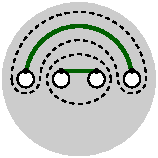
\includegraphics[]{pic-2-curve.pdf}
\end{center}
The bijections works as follows.
To construct a $2$-observable from a $2$-curve $c$ that
joins two holes $M_1$ and $M_2$,
take a small neighbourhood of
the union $c([0,1])\cup M_1 \cup M_2.$
This neighbourhood will have boundary a simple closed
curve that encloses $M_1$ and $M_2.$
\emph{(is this really how to prove this? do we care?)}
\emph{(check the orientation of the $2$-observable has the correct interior)}
Going the other direction we can take
any $2$-curve contained within the interior of a $2$-observable,
\emph{but how do we show these are all isotopic?}

%The end points of $2$-curves are free to terminate anywhere
%on the hole, but we can fix the endpoints using
%the base points.
%A simple way to do this is to just require the
%$2$-curve to begin and end on base points.


A single $F-$move is seen to relate a pair of $2$-curves
that share a hole.
Continuing in this way, we can chain these $2$-curves together:
\begin{center}
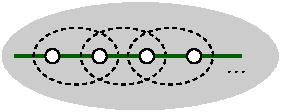
\includegraphics[]{pic-chain.pdf}
\end{center}

We call such a chain a ``linear order''.
This will be unique up to Dehn-twists around holes.
Also, the curve is directed according to the direction
of the constituent $F-$moves.

Clearly there are many ways to do this, up to isotopy.
Remarkably, we can generate (switch between)
all possible linear orders using 
a single linear map (and extension under gluing)
called the $R-$move.
This is a (collection of) linear operator(s)
$R^{ab}_c:V^{ab}_c\to V^{ab}_c$
whose action on linear orders is depicted as follows:
\begin{center}
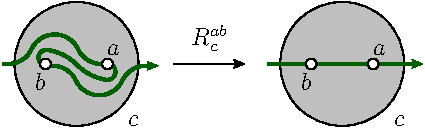
\includegraphics[]{pic-rmove-1.pdf}
\end{center}

At this point we can show the relation to skein theory:
\begin{center}
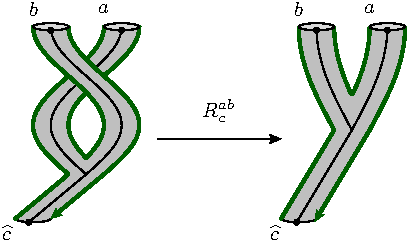
\includegraphics[]{pic-rmove-skein.pdf}
\end{center}
This diagram is intended to be the same as the previous flat
diagram,
with the addition of a third dimension, and also thin black lines
connecting the marked points.
The black lines do not add any extra structure, they can
be seen as a part of the dual of the ``hexagon'' cut out by
the green line and boundary components.

We can try to pluck the linear
operator $R^{ab}_c:V^{ab}_c\to V^{ab}_c$
directly out of the
modular functor by considering a half twist
$\sigma$ that swaps the $a$ and $b$ component.
This is a diffeomorphism $\sigma:M^{ab}_c\to M^{ba}_c$
which the functor sends to a 
linear map $\F(\sigma):V^{ab}_c\to V^{ba}_c.$
Therefore, unless $a=b$ (or $a=\vac$ or $b=\vac$)
this fails to give the $R-$move we sought.

We can get monodromy operators, and theta operators...

Digging a bit deeper in looking for $R-$moves,
we seek something that
appears to be a collection of natural transformations of $\F,$
one $R^{ab}_c$ for each pair of pants $M^{ab}_c.$
The naturality requirement says that
the $R-$moves commute with (linear maps induced by) diffeomorphisms.
In more detail,
given any diffeomorphism
$f:M^{ab}_c\to M^{\tilde{a}\tilde{b}}_{\tilde{c}}$
we have $\F(f)R^{ab}_c=R^{\tilde{a}\tilde{b}}_{\tilde{c}}\F(f).$
Here is an example of this, with $f$ a counter-clockwise half twist
$f:M^{ab}_c\to M^{ba}_c:$
\begin{center}
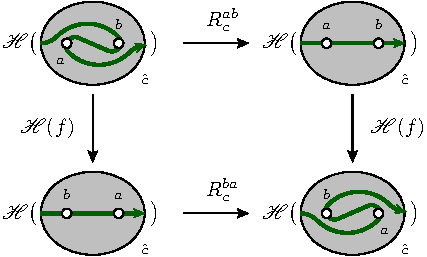
\includegraphics[]{pic-natural.pdf}
\end{center}
It is not clear how to extend this to
a collection of maps for all possible surfaces, as is
required to be an actual
natural transform of $\F.$
However, such a natural transform would be notated as 
%category theorists would write this as
$ R^{ab}_c : \F\to\F,$
and this looks good because natural transformations
can be thought of as $2-$morphisms (a morphism of morphisms) and we
do expect the braiding to be somehow one level up
in the $n-$categorical sense.

The following commutative triangles show two
relations among possible $F-$moves on a 3-punctured
disc:
\begin{center}
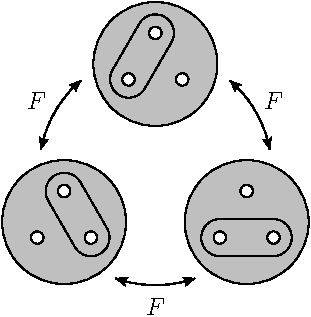
\includegraphics[width=0.2\columnwidth]{pic-fmove-relation.pdf}
\ \ \ \ \ 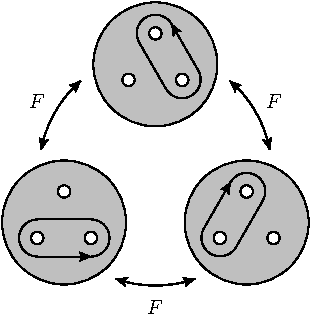
\includegraphics[width=0.2\columnwidth]{pic-fmove-relation-r.pdf}
%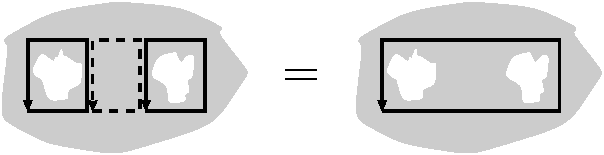
\includegraphics[width=0.4\columnwidth]{pic-abelian.pdf}
\end{center}

The $R-$move maps between each of these
three $F-$moves, and so the
following hexagonal diagrams must commute:
\begin{center}
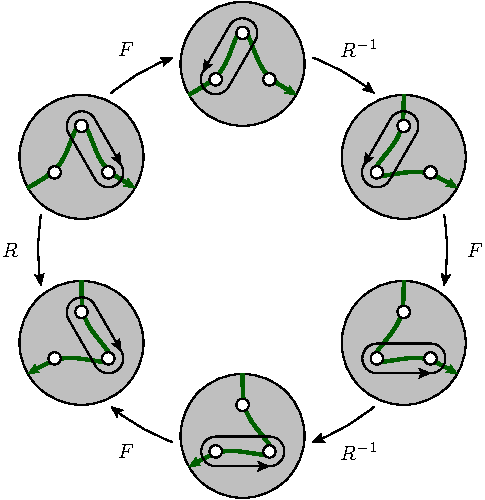
\includegraphics[width=0.3\columnwidth]{pic-hexagon.pdf}
\ \ \ \ 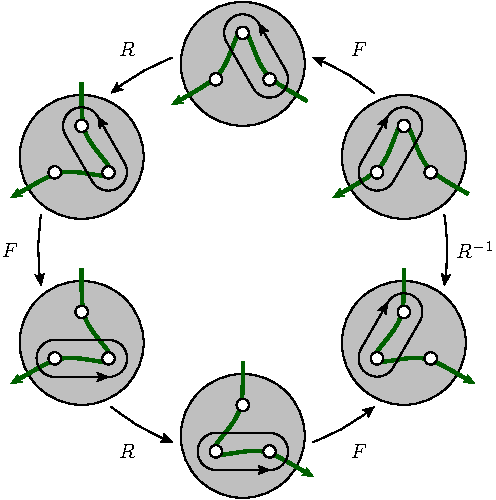
\includegraphics[width=0.3\columnwidth]{pic-hexagon-r.pdf}
\end{center}
Note that we don't fix the framing.
The symmetry of this equation becomes evident when
the four holes are arranged at the vertices of a regular
tetrahedron.

What we have done here is show how the skein theory of
braided tensor categories arises from a modular functor.
This does not seem to be written down anywhere in any
detail: Turaev \cite{Turaev1994} derives a Ribbon category
from his definition of a modular functor, but this
definition is different to the one given here, which is
based on \cite{Walker1991}, and is not known to be equivalent.
Walker \cite{Walker1991}
(and others \cite{Bakalov2000}) perform the much more
difficult task of deriving a modular functor from
algebraic data (braided tensor category, etc.)
but do not seem to say much about going in the other direction.

%
% ~~~~~~~~~~~~~~~~~~~~~~~~~~~~~~~~~~~~~~~~~~~~~~~~~~~~~~~~~~~~~~~~~~~~~~~~~~~~
%

%\section{The refactoring theorem}
%
%
%  XXX useless
%\begin{center}
%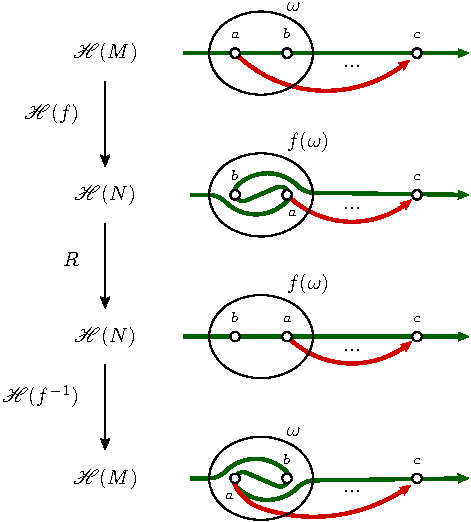
\includegraphics[]{pic-refactoring.pdf}
%\end{center}

%
% ~~~~~~~~~~~~~~~~~~~~~~~~~~~~~~~~~~~~~~~~~~~~~~~~~~~~~~~~~~~~~~~~~~~~~~~~~~~~
%

\section{Combinatorial curve diagrams}

The basic data structure involved in the
simulation we term a \emph{combinatorial curve
diagram.}
% XXX define "piece of curve"
Firstly, we will require each curve to intersect 
the edges of tiles transversally,
and in particular a curve will not touch a tile corner.

For each tile in the lattice,
we store a combinatorial
description of the curve(s) intersected with that tile.
Each component of such an intersection we call a \emph{piece-of-curve.}
\begin{center}
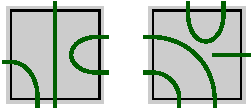
\includegraphics[]{pic-cells.pdf}
\end{center}

We follow essentially the same approach as taken in \cite{Abramsky2007} 
to describe elements of a Temperley-Leib algebra, but
with some extra decorations.
The key idea is to store a \emph{word} for each tile, comprised of
the letters $\bigl<$ and $\bigr>$.
%The encoding works as follows.
Reading in a clockwise direction around the edge of
the tile from the top-left corner,
we record our encounters with each piece-of-curve,
writing~$\bigl<$ for the first encounter, and~$\bigr>$ for the
second.
We may also encounter a dangling piece-of-curve
(the head or the tail), so we use another symbol $*$ for this.
The words for the above two tiles will then be 
$\bigl<\bigl<\bigr>\bigr>\bigl<\bigr>$ and $\bigl<\bigr>*\bigl<\bigl<\bigr>\bigr>.$
When the brackets are balanced,
each such word will correspond one-to-one with an intersection
of a curve in a tile, up to a continuous deformation of the interior of the tile.
Ie. the data structure 
will be insensitive to any continuous deformation of the interior of the tile,
but the simulation does not need to track any of these degrees of freedom.

\begin{center}
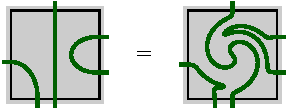
\includegraphics[]{pic-cells-0.pdf}
\end{center}

We will also need to record
various other attributes of these curves,
and to do this we make this notation more elaborate
in the paragraphs {\bf (I)}, {\bf(II)} and {\bf(III)} below.
Each symbol in the word describes an intersection of
the curve with the tile boundary,
and so as we decorate these symbols these decorations will
apply to such intersection points.

\begin{center}
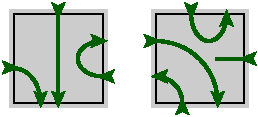
\includegraphics[]{pic-cells-1.pdf}
\end{center}

{\bf (I)} We will record the direction of each piece-of-curve,
this will be either an {\tt in} or {\tt out} decoration for each symbol.
Such decorations need to balance according to the brackets.
The decorated symbols $*_{\mbox{\tt in}}$ and 
$*_{\mbox{\tt out}}$ 
will denote respectively either
%the head, $c(1)$ or the tail $c(0)$ of a curve.
the head or the tail of a curve.
The words for the diagrams above now read as
$ \bigl<_{\mbox{\tt in}}\bigl<_{\mbox{\tt out}}\bigr>_{\mbox{\tt in}}
    \bigr>_{\mbox{\tt out}}\bigl<_{\mbox{\tt out}}\bigr>_{\mbox{\tt in}}$
and
$ \bigl<_{\mbox{\tt in}}\bigl>_{\mbox{\tt out}}*_{\mbox{\tt in}}
    \bigr<_{\mbox{\tt out}}
    \bigr<_{\mbox{\tt in}}\bigl>_{\mbox{\tt out}}\bigr>_{\mbox{\tt in}}.
$

{\bf (II)} We will record,
for each intersection with the tile edge, 
a numeral indicating which of the four
sides of the tile the
intersection occurs on.
Numbering these clockwise from the top as $1, 2, 3, 4$ we have for the above curves: 
$\bigl<_1\bigl<_2\bigr>_2\bigr>_3\bigl<_3\bigr>_4$ 
and $\bigl<_1\bigr>_1*_2\bigl<_3\bigl<_3\bigr>_4\bigr>_4.$

{\bf (III)} Finally, we will also decorate these symbols with anyons.
This will be an index to a leaf of a (sum of) fusion tree(s).
This means that anyons only reside on the curve close
to the tile boundary,
and so we cannot have more than two anyons
for each piece-of-curve. 
The number of such pieces is arbitrary, and so this
is no restriction on generality.

\begin{center}
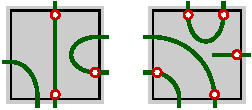
\includegraphics[]{pic-cells-2.pdf}
\end{center}

In joining tiles together to make a tiling we will
require adjacent tiles to agree on their shared boundary.
This will entail sequentially pairing symbols in the
words for adjacent tiles
and requiring that 
the {\tt in} and {\tt out} decorations are matched.
Because the word for a tile proceeds conter-clockwise
around the tile, this pairing will always reverse the
sequential order of the symbols of adjacent tiles.
For example, given the above two tiles we sequentially pair the 
$\bigl<_{\mbox{\tt out},2}\bigr>_{\mbox{\tt in},2}$ 
and $\bigr>_{\mbox{\tt out},4}\bigr>_{\mbox{\tt in},4}$
symbols with opposite order so that
$\bigl<_{\mbox{\tt out},2}\sim\bigr>_{\mbox{\tt in},4}$
and $\bigr>_{\mbox{\tt in},2} \sim \bigr>_{\mbox{\tt out},4}.$ 

%Two other consistency relations are enforced on such a combinatorial curve diagram:
%we require adjacent tiles to agree on their boundaries, 
%and every curve diagram
%must have two ends.
%One final consistency
%relation is enforced by requiring 
%We require every curve diagram to have two ends, this means
%that there are no loops.

Note that in general this data structure will store many disjoint curve diagrams
$c_i:[0,1]\to D_{n_i}$ within a disc $D_m$ where $\sum n_i = m.$

%For a given piece-of-curve, we can subtract the numeral with
%the {\tt in} label from the numeral with the {\tt out} label
%to get an integer in $\{ \}$ WRONG
%We can also just use the numerals of the boundary edges
%that the piece-of-curve intersects with, subtracting the
%``exit'' boundary numeral from the ``entry'' boundary numeral. WRONG

For each piece-of-curve, apart from a head or tail, there is an associated 
number we call the \emph{turn number}. This counts the number
of ``right-hand turns'' the piece-of-curve makes as it
traverses the tile, with a ``left-hand turn'' counting as $-1.$
(To be more rigorous, we would define this number using the
winding number of the simple closed curve formed by the
piece-of-curve adjoined to a segment of the boundary of the tile 
traversed in a clockwise direction.)
This number will take one of the values $-2, -1, 0, 1, 2:$
\begin{center}
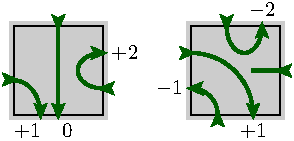
\includegraphics[]{pic-cells-3.pdf}
\end{center}


%Two disjoint curves can be joined by...
%
%Curves can be simplified along sections without any anyons, ...

% Each piece will have +1, +2, 0, -1, -2 right-hand turns...

% mention Jones' planar algebras ?

%
% ~~~~~~~~~~~~~~~~~~~~~~~~~~~~~~~~~~~~~~~~~~~~~~~~~~~~~~~~~~~~~~~~~~~~~~~~~~~~
%

\section{The paperclip algorithm}

Anyons are transported around the lattice
by moving them along tile edges.
In general, such a transport will intersect with a
curve diagram in many places.
Each such intersection is transverse,
and we use each intersection point to cut
the entire transport into smaller paths each of
which touch the curve diagram twice.
%Each intersection with a curve diagram
%will then be transverse, and we
%decompose the entire path into a sequence of
%paths each of which 
%join consecutive intersections.
%Transport of an anyon can be decomposed into
%moves between adjacent components of a curve
%diagram.
The origin and destination of such an anyon path
now splits the curve diagram $c:[0, 1]\to D_n$ 
into three disjoint pieces which we term
\emph{head}, \emph{body} and \emph{tail}, where
the head contains the point $c(1)$, the tail
contains $c(0)$ and the body is the third piece.
These arise with various arrangements, but here
we focus on one instructive case, the
other cases are similar:
%We look at the particular case of moving along
%one edge of a tile,
transporting along one edge of a tile \emph{forwards} 
(from tail to head) along a curve diagram:
\begin{center}
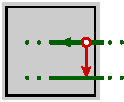
\includegraphics[]{pic-move-anyon.pdf}
\end{center}

This arrangement is equivalent (homotopic) to one of four 
``paperclips'', which we distinguish between by counting how
many \emph{right-hand turns} are made along the body of the curve diagram.
We also show an equivalent (homotopic) picture where the
curve diagram has been straightened, and the resulting distortion
in the anyon path:
\begin{center}
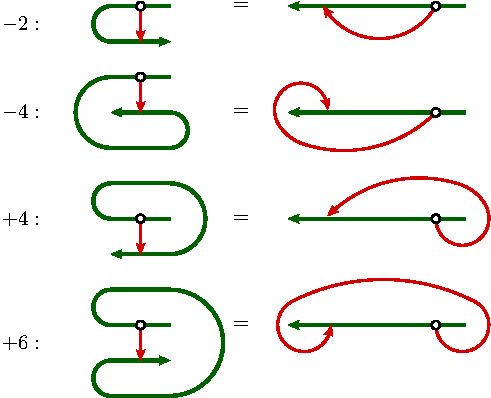
\includegraphics[]{pic-paperclip.pdf}
\end{center}
The sequence of anyons along the head, body and tail, we denote as $H, B$ and $T,$
respectively.
These sequences have the same order as the underlying curve diagram, and 
we use
$H^r, B^r$ and $T^r$ to denote the same anyons with the reversed order.
Using the above diagram, we can now read off the $R$-moves for each
of the four paperclips:
\begin{align*}
-2:&\ R[B] \\
-4:&\ R[H^r]\ R[H]\ R[B] \\
+4:&\ R[B]\ R[T]\ R[T^r] \\
+6:&\ R[H^r]\ R[H]\ R[B]\ R[T]\ R[T^r] \\
\end{align*}
where notation such as $R[B]$ is understood as sequentially clockwise braiding around
each anyon in $B$.

That these four paperclips exhaust all possibilities can be seen by
considering the winding number of the simple closed curve made
by combining the body of the curve diagram with the path followed by
the anyon (appropriately reversing direction as needed).


%\section{Computation of homologically non-trivial operators}\label{s:homnontrivial}
%
%Specializing to the Fibonacci case,
%we write the non-trivial $F$-moves as the following
%skein relations:
%\begin{align*}
%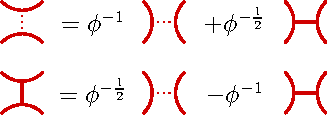
\includegraphics[]{pic-skein1.pdf}
%\end{align*}
%
%The sollid lines represent Fibonacci world-lines.
%The dotted lines represent vacuum charges,
%and we are free to include these lines or not.
%We leave these anyon paths
%as undirected because Fibonacci anyons are
%self-inverse.
%The non-trivial $R$-moves are:
%\begin{align*}
%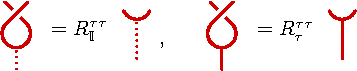
\includegraphics[]{pic-skein2.pdf}
%\end{align*}
%
%Removing bubbles:
%\begin{align*}
%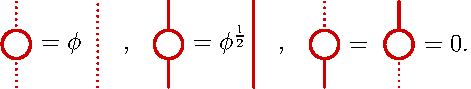
\includegraphics[]{pic-bubble.pdf}
%\end{align*}
%
%Here we show a process where a 
%Fibonacci anyon travels around the torus and
%anihilates itself. Twice.
%The vertical lines represent a periodic
%identification.
%\begin{align*}
%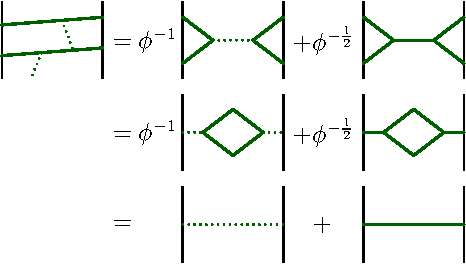
\includegraphics[]{pic-logops.pdf}
%\end{align*}
%
%The state is not normalized.
%Also involves post-selection, as there is
%another process that involves leakage...
%The first equation is an $F$-move, 
%the second equation is a translation in the
%horizontal direction, and the last equation
%follows from the rule for collapsing bubbles.
%
%Continuing in this way, we compute the $k$-fold
%logical operator:
%\begin{align*}
%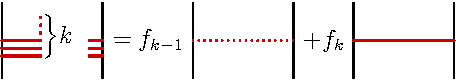
\includegraphics[]{pic-kfold.pdf}
%\end{align*}
%
%where $f_k$ is the $k$-th element of the Fibonacci
%sequence $\{1, 1, 2, 3...\}.$


%------------------------------------------------------------------------------------------------------------%
\bibliography{refs2}



\end{document}
